%!TEX root = thesis.tex

\chapter{Related work}
\label{chap:rw}

I found and studied a large number of research papers as part of the literature review stage of this project. When I started the review, I already had a good starting point on what specifically to research, because had known that my focus would be restricted to three specific, openly available Dutch geospatial datasets, and because I had already settled on a range of specifics regarding the goals and requirements of the project. The three datasets were picked early on in the planning process for reasons related to our wish to mainly use the same datasets as the commercial solution does.

As it is the most up-to-date detailed elevation source, and thus suitable for performing detailed surface modelling in addition to the 3D conversion of lines, my primary candidate became the national \ac{als} point cloud of The Netherlands. The name of the latest release of this product is abbreviated \ac{ahn3}. As a result of this choice, there are two main areas that I focused on as part of my literature review: road feature reconstruction from Lidar point clouds, and the theoretical and empirical propagation of Lidar accuracy into derived models. The literature review concerning these two areas is presented below in two independent parts.

The other two datasets are \ac{nwb} itself, and a 3D line dataset called \ac{dtb} which has coverage in many areas where \ac{ahn3} does not. Detailed information about the choices regarding the datasets, as well as an analysis about their detailed properties, can be found in in Section \ref{sec:input}.

\section{Road identification in point clouds}
\label{sec:roadidentification}

My main domain of interest was feature extraction from Lidar data, because tasks of this type characterised the bulk of the planned processing pipeline. Our intention was to not only query a \ac{dtm} for elevations around the \ac{nwb} road centrelines - an example of a simple way in which one could perform a \textit{rudimentary} 3D conversion - but to create spatial models of road edges and surfaces, and only then proceed to extracting elevations for the centrelines. This requires one to identify, or at least approximate the geometries of these features by choosing the point cloud points that best describe them and applying various operations to them.

We may thus regard point cloud feature extraction as the top-level geomatics topic concerned by this research, with most other operations, such as 2.5D surface modelling and mathemamatical tools, as residing a level lower in the hierarchy. We are using them for the purpose of identifyng and modelling discrete physical features found in the point cloud (and the support dataset, which will be discussed later in this chapter).

\subsection{Research using point clouds only}
\label{sub:roadidentification_pconly}

\subsubsection{Approaches based on photogrammetry}

In terms of point cloud feature extraction techniques relevant to roads specifically, I studied a range of papers detailing a wide spectrum of methods. One strategy, most prominently represented by \cite{hu_2003, hu_etal_2004, zhu_mordohai_2009, zhu_hyppa_2014, lin_etal_2015}, is based on the idea of transitioning to a photogrammetric analysis at some point in the process, generally quite early on. First, a set of pre-processing techniques to better characterise potential road points in the source Lidar data are applied, generally by performing some form of filtering (e.g. setting intensity thresholds applicable to Lidar returns from bitumen), or by extracting ground planes using various techniques and selecting points that lie close to them. Then, images are rendered from the point cloud from various angles, often using colour-coding based on point properties, and applying photogrammetric methods to identify roads. Sometimes, high-definition aerial or satellite imagery is incorporated in the photogrammetric workflows. The success rates of such strategies are mediocre, and they rely strongly on manual parametrisation. In particular, they are unsuitable for large study areas with inhomogeneous types and distributions of roads, as also concluded by the excellent review of this type of relevant work in the literature review section of the paper \cite{yang_etal_2013}.

\subsubsection{Approaches based on curb detection}

A further popular set of strategies rely on road curb detection. \cite{vosselman_zhou_2009}, \cite{zhang_2010}, and \cite{yang_etal_2013} are examples of such research. \cite{vosselman_zhou_2009} presents a method in which a \ac{dtm} is generated, points close to its surface are selected from the point cloud and small, curb-like jumps in elevation are algorithmically detected using thresholds. The curb points are selected, and a feature extraction method (\ac{ransac} in this case) is used to construct 3D lines from them. Gaps in the lines are closed procedurally, and B-splines are fitted to optimise the shapes of the road edges. In \cite{zhang_2010}, road cross-sections are constructed and inspected in 1D, and points are "classified" based on whether they are likely to represent road surfaces, curbs, or off-road surfaces. To do this, they process \ac{mls} data on-the-fly (during acquisition) via a supervised classifier, and use the Hough transform to model the road surface. The curbs are found where the points first deviate from the model.

In \cite{yang_etal_2013} a similar approach is presented in which cross-sections are identified by looking at \ac{mls} scan properties (time of acquisition, specifically), and then non-road points are filtered out in 1D based on the absolute elevation of the road (known from constant elevation of the sensor above it) and curbs \textit{of a specific type} are identified in the 1D series of ground points - all via a single moving-window operation that uses applicable thresholds.

While the results of the curb detection-based methods are more flexible, more accurate and more complete in general than the photogrammetric methods, they are not well suited for my project out-of-the box. These approaches work best with \ac{mls} data, where the data is either natively produced in the form of road cross-sections (the scan lines of a car-mounted front facing sensor), or can be easily extracted from the point cloud in such a form. Furthermore, in \ac{mls} sensing the road elevation is generally known, by considering the sensor's constant position relative to the vehicle's \ac{gnss} sensor - this is not the case in \ac{als}. Lastly, while the above method may work well in places where curbs are well-defined, this is not a reasonable assumption to make for an \ac{als} dataset with nationwide coverage, such as our particular input.

The work \cite{vosselman_zhou_2009} is not entirely bound by the above limitations. It demonstrates that a relatively simple approach can be used to detect curbs without the need for the point cloud to be comprised natively of cross-sections, and for accurate road elevations to already exist. However, the fact that it also uses curb detection with fixed thresholds undermines my confidence in it. Working with a national dataset and focusing on large roads (including motorways, one of our main targets for 3D conversion) means that the assumption that well-defined, relatively uniform road curbs will exist and be reliably detectable everywhere is not a sensible assumption.

\subsubsection{Other, purely Lidar-based approaches}

There are many other papers that deal with this task without relying on external vector data. For instance, \cite{clode_etal_2004} and \cite{clode_etal_2007} present a set of methods in which first a \ac{dtm} is generated, then points close to the \ac{dtm} are selected and are further filtered based on intensity and sampling density thresholds applicable to reflections from flat bitumen surfaces. The results are converted to a raster mask which is then refined via morphological operations. It is then used to produce the output: a point cloud in which road points are marked semantically (i.e. they are classified as such). In the 2007 paper, they extended the procedure by convolving the results with a \ac{pcd}, which can create a 2D map of the predicted road parameters wherever it moves through road points. Like the morphological operations above, the \ac{pcd}-convolution is in fact a photogrammetric method, because it also acts on a raster generated from the classified point cloud prior to its application. Nevertheless, the method is still more relevant to us than the rest of the photogrammetry-based research mentioned here. An example visualisation of its output is shown in Figure \ref{fig:phasecodeddisk}, the vector magnitude in any given pixel quantifies the support that exists there for the presence of a road centreline - it is effectively a centreline detector. They describe it as an alternative to using the Hough-transform for finding road centrelines, which, according to their research, is not reliable enough in this context. This spatial map can then be used to generate a vector dataset describing the geometry of the roads.

\begin{wrapfigure}[20]{O}{0.48\linewidth}
    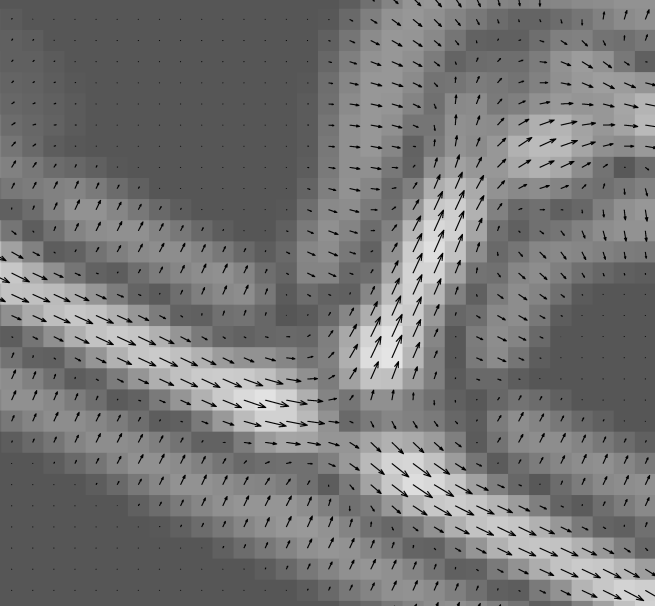
\includegraphics[width=\linewidth]{final_report/figs/clode_etal_2007_01.png} 
    \caption{Illustration of the results of \ac{pcd} convolution from \cite{clode_etal_2007}.}
    \label{fig:phasecodeddisk}
\end{wrapfigure}

The research \cite{gross_thoennessen_2006} shows that point neighbourhood information can be used to generate covariance matrices of individual points, which can in turn be used directly to indicate if the point belongs to a linear feature. They also describe how lines can be assembled from the selected points efficiently. Although their methods have very well documented mathematical foundations which could be reproduced in any programming language, their applicability in my research, especially in the context of small or even non-existent curbs, is uncertain.

Other methods relying purely on the Lidar points themselves exist, but like \cite{zhang_2010}, they are typically intended for real-time \ac{mls} applications - such as the fully convolutional neural network-based solution in \cite{caltagirone_etal_2017}. The literature review in \cite{yang_etal_2013} offers an excellent overview of such additional methods, but they will not be described here any further, as I found them not to be relevant to this project.

\subsection{Research using input point clouds and approximate road locations}
\label{sub:lidaraccuracy_external}

This section contains brief descriptions of research that used similar input data to mine \textit{in addition to} Lidar data; mainly vector datasets estimating road centreline positions. These relevant papers describe work that used analogous input data to achieve similar goals to mine - as a result, they contain the methods that are the most relevant to my own research.

\subsubsection{Relatively simple approaches}

The work \cite{hatger_brenner_2003} presents two approaches based on region-growing. The first one is based on growing planes in the entire study area from Lidar points. Finding this to be too complex computationally, they propose another approach of treating Lidar scan lines individually, partitioning each into parametrised line segments via linear regression and then inspecting the succession of scan lines and identifying neighbouring segments that are roughly parallel. The resulting groups of (roughly parallel) 3D lines are then treated as cross-sections of planar regions, and an additional region growing step is performed to find any points that might have been left out in the previous steps. The results of this can then either be prepared as a full, 3D planar partition of the study area onto which road polylines can simply be projected, or they can be further refined first by eliminating small, meaningless planes via a \ac{ransac}-based workflow.

The work \cite{cai_rasdorf_2008} shows that enriching road centrelines with elevations can be achieved using even more simplistic methods. Their first method is based on finding points on opposite sides of roads (in 2D) at similar distances from them, and in suitable locations to form approximate cross-sections. The centrelines are intersected with the cross-sections and are given elevations at the points of intersection. The elevations are computed by interpolating linearly inside the cross-sections, using the elevations of the two points that define each of them. Their second method is even simpler; for each road vertex  (or some sampling along its length), they locate the closest Lidar point and associate its elevation with it. The simplicity of these methods is reminiscent of the \ac{ndw} prototype and the commercial solution developed for \ac{ndw} by \ac{rhdhv} (described in Section \ref{sec:methodsexisting}), and highlights that a rough approximation for the road elevations can, in practice, be made either directly from the point cloud or from a derived \ac{dtm} in a straightforward manner. However, far more sophisticated methods have been developed by other authors.

\subsubsection{Complex approaches based on active contour optimisation}

One landmark paper, \cite{boyko_funkhauser_2011}, describes a method in which a set of 2D input LineStrings are used to identify and label road points in an \ac{als} point cloud. The input lines contain road intersection nodes and patches, from which centrelines are derived. They first associate the input lines with elevations by fitting spline curves through Lidar points close to the centrelines in 2D. Suitable Lidar points are selected by minimising an error function that includes terms related to the distance from the location of interpolation, and to elevation variance. The resulting network is guaranteed to be continuous and smooth because the densified input polylines are used as spline control points. Since the entire system of splines is connected, this is also guaranteed to minimise the effects of local issues, such as occlusion.

\begin{figure}
    \centering
    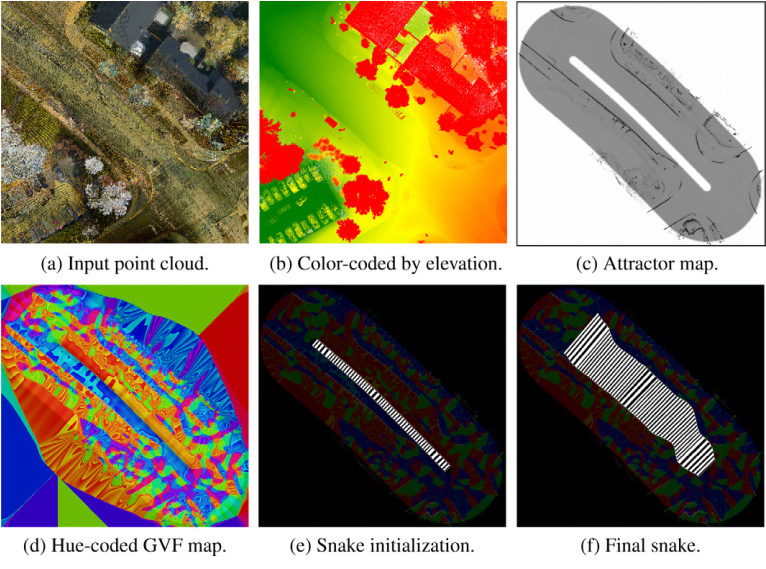
\includegraphics[width=0.85\linewidth]{final_report/figs/boyko_funkahuser_2011_01.png} 
    \caption{Illustration of the contour optimisation procedure used in \cite{boyko_funkhauser_2011}.}
    \label{fig:boykofunkhauser2011}
\end{figure}

The point cloud is then partitioned on disk, based on fitting support planes along the 3D-converted lines and fetching points that are close to them, solving performance-related issues of working with too many Lidar points at once, and further minimising the effects of 2.5D violations related to overlapping features. They then construct scalar maps for each resulting segment that penalises points away from road edges (both inwards and outwards). These maps, called attractor maps, are composited from rasters penalising locations that are outside the range in which edges are expected to be found (relative to the centrelines), and rasters produced by a curb detection metric related to the normal vectors of the point cloud points. Lastly, they apply an active contour optimisation technique (specifically, ribbon snakes) that yields the road edges in 3D, and then labels points between the two edges as road points. An illustration is shown in Figure \ref{fig:boykofunkhauser2011}, taken from their paper. In the attractor map, darker colours represent stronger attraction, resulting in the active contour converging to them in the optimisation procedure. The GVF map is a vector map that contributes to favourable active contour convergence and is not described any further here (please refer to the original paper). The initial contour is based on the road centreline (from external vector data).

The results of \cite{gopfert_etal_2011} demonstrate that active contour optimisation can be used to estimate road outlines without the need for the involved pre-processing steps of \cite{boyko_funkhauser_2011}. They convert the input point cloud directly into a \ac{dtm}, and then into attractor maps. They use the same general type of active contour optimisation, and generate output centrelines and road edges with comparable quality to that of the outputs of \cite{boyko_funkhauser_2011}. It is worth mentioning that the type of active contour optimisation used by these two papers also optimises the road centrelines in conjunction with the road edges, which is particularly important in places where the 2D georeferencing of the original centrelines is poor.

\subsubsection{Relevant work with Dutch data}

The work \cite{oudeElberink_vosselman_2006} is relevant not only because of the methods it applies, but also the specific datasets. They enrich the best-known Dutch open data national topographical vector dataset (the present-day equivalent of which is \ac{bgt}) with elevations, and as their source of elevations, they use \ac{ahn} data (the first edition of \ac{ahn}, the third edition of which I used in my own research).

\begin{wrapfigure}{O}{0.5\textwidth}
    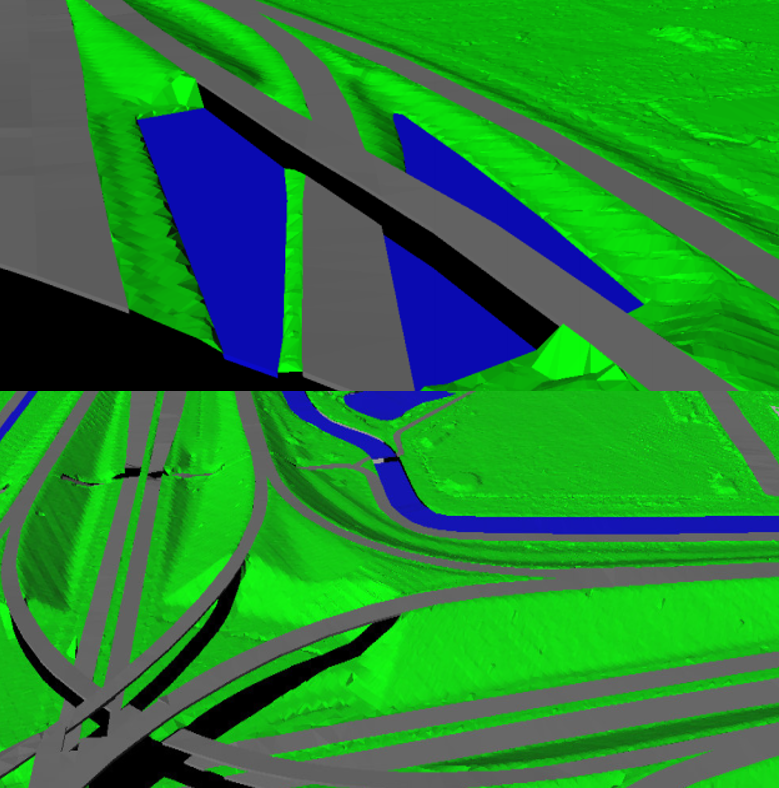
\includegraphics[width=\linewidth]{final_report/figs/oudeElberink_vosselman_2006_03.png} 
    \caption{Examples of 3D-converted multi-level road vector geometry from \cite{oudeElberink_vosselman_2006}.}
    \label{fig:conversionartefacts}
\end{wrapfigure}

They do not exclusively consider roads; all polygonal vector objects are extruded to 3D. Like in \cite{hatger_brenner_2003}, a region growing approach is proposed as the foundation of the elevation extraction workflow. They use the Hough transform to find seed points whose neighbourhood suggests a planar structure, fit planes and then grow them by checking the point-to-plane distance of new points, labelling points with the identifier of the plane they belong to. The vector data is then overlain on these regions and for each polygon, the plane is selected which is represented by the greatest number of labelled points in its interior. These points are re-fitted a plane, and each such plane is used to extrude the corresponding overlain vector geometry simply by projecting the polygon onto its surface. To improve upon the results of this simple extrusion, they suggest the application of algorithmic topological corrections. Furthermore, to model the interior of the extruded polygons in more detail, they recommend the construction of a \ac{cdt} for each, first by inserting its edges as constraints, and then by inserting the Lidar points that its surface is based on. The \ac{cdt} can be refined procedurally to ensure smoothness. The main limitations of their methods are that the extracted elevations (from the region growing approach) are not reliably accurate, and that it cannot handle overlapping objects, such as roads in motorway junctions. 3D visualisations of the results of this approach and typical artefacts are shown in \ref{fig:conversionartefacts}. The specific artefacts shown in the figure demonstrate that in multi-level road layouts, only the topmost road is fully converted to 3D.

Their method was later extended in \cite{oudeElberink_vosselman_2009} to work well in complex multi-level road settings by using point cloud segmentation in a manner resembling what I already described in the context of \cite{boyko_funkhauser_2011}, which we may regard in general as decomposing the 3D problem into 2.5D sub-problems, also a main aim of my own research. In his doctoral thesis \cite{oudeElberink_2010} he combined this method with the overall procedure in \cite{oudeElberink_vosselman_2006} to form one integral whole. Furthermore he extended it with a road extraction quality and accuracy assessment procedure, which was later perfected and also published separately in \cite{oudeElberink_vosselman_2012}.

Their quality and accuracy assessment methodology is comprised of two separate procedures and the comparison of their results: a theoretical (error propagation-based) evaluation, and an empirical one against reference data. Their error propagation-based evaluation takes into account metrics such as \ac{gnss} and \ac{ins} noise in the Lidar survey (suggesting that they had access to low-level information about the dataset), plane fit quality and observed Lidar noise. It also considers interpolation/extrapolation uncertainty, relevant in places where not enough relevant Lidar points could be located and thus such gap-filling measures were used. They found that these theoretical errors were generally below 20 cm, with noticeable increases only occurring where Lidar coverage was extremely sparse or non-existent, leading to the necessity of using interpolation or extrapolation. 

Interestingly, their reference data was \ac{dtb} for the empirical evaluation of accuracy, which is also the support dataset I used in my research (see Section \ref{sub:dtb}). In general, their comparison with \ac{dtb} showed good agreement with their road surface extraction results, except for the same places where the theoretical approach also suggested large errors, and in particular in places where this was also combined with intense vertical road curvature locally, which \ac{dtb} managed to capture, but not their results. In places with good Laser coverage, the agreement was much better, often near-perfect. Although not explicitly mentioned, it appears that they still used the earliest version of \ac{ahn} (not \ac{ahn2}) in this research, which may explain how it is possible that they encountered low point densities even in well-exposed road segments. \ac{ahn2} and \ac{ahn3} no longer have this problem, as mentioned in \ref{sub:ahn} and in many other subsequent parts of this report.

\subsubsection{On using a support dataset in addition to Lidar data}

In Section \ref{sec:input} in this chapter, I discuss that this research is also concerned with  another source of elevations, which I often refer to as the "support dataset" in this report because \ac{ahn3} is given priority to in the analysis, wherever it exists. It is a 3D line dataset, not an \ac{als} or \ac{mls} point cloud. The one area \textit{not} explicitly covered in any of the papers I examined is the use of such external 3D vector data as a further constraint when extracting road elevations and/or geometries from point clouds.

In relevant work, occlusion is generally accepted to represent gaps in coverage, and elevations are simply interpolated or extrapolated inside them if possible - or if not, they are not considered any further. In the case of my research, \ac{ndw} is interested in producing a 3D conversion of \ac{nwb} with the highest possible \textit{completeness}. Exploring how information from the two datasets can be combined is also interesting academically, thus my work will examine how \ac{dtb} can be used to patch in gaps in \ac{ahn3} coverage. While doing so, I will be building solely on my own ideas, as I could not find work that is directly relevant to this topic.

\section{Lidar accuracy and sampling density}
\label{sec:lidaraccuracy}

Relevant aspects of Lidar-related accuracy assessment can be divided into two main sub-topics: interpreting the reported global and/or local accuracy and areal sampling density of the Lidar surveys themselves, and assessing the accuracy of terrain models that one may derive from Lidar point clouds, and the elevations that can be interpolated from them. Although some of the relevant work I studied overlaps with both of these areas, I separated the discussion below into two sections based on them. As Lidar sensing accuracy and sampling density underlies that of the derived models, I discuss it first below.

\subsection{Accuracy description of Lidar sensing}
\label{sub:lidaraccuracy_sensing}

\subsubsection{Global and local influences on accuracy}

\begin{wrapfigure}{O}{0.44\textwidth}
    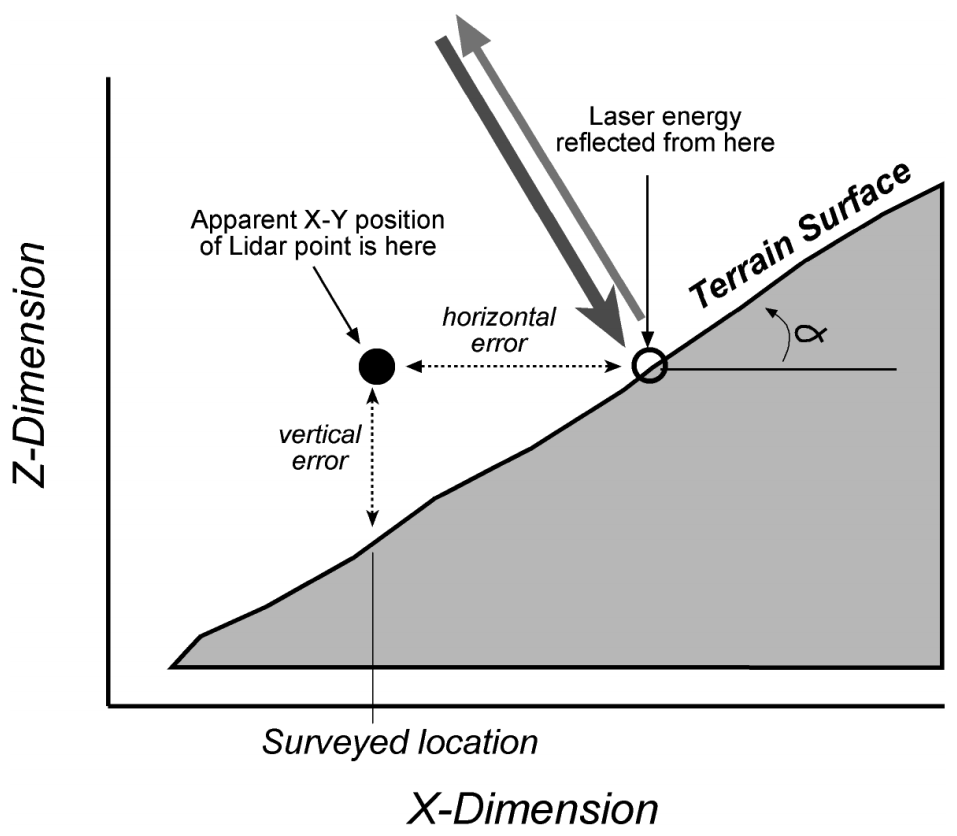
\includegraphics[width=0.95\linewidth]{final_report/figs/hodgson_breshanan_2004_01.png} 
    \caption{Illustration of the effects of terrain slope on vertical accuracy from \cite{hodgson_breshanan_2004}.}
    \label{fig:elevationaccuracy}
\end{wrapfigure}

Many papers describe that the accuracy of Lidar-derived \ac{dtm}s depends primarily on the accuracy of the sensing method itself. The notable paper \cite{hodgson_breshanan_2004} describes the most fundamental sensing errors of Lidar measurements to be introduced by \ac{gnss} errors, \ac{ins} errors, \ac{imu} errors, errors introduced by the waveform analysis algorithm and lastly, a general error factor that depends on the flying height. Combined, these are the primary factors that contribute to the \textit{measurement} accuracy of the sensing system.

It is shown by various papers including \cite{hodgson_breshanan_2004, su_bork_2006, kraus_etal_2006, raber_etal_2007, peng_shih_2006, chow_hodgson_2009, aguilar_etal_2005, aguilar_etal_2010, guo_etal_2010} that there are local factors influencing \textit{vertical} Lidar accuracy that are independent of the sensing equipment, and thus vary from survey to survey. In production datasets, whether they are considered at all or not, they are almost never \textit{reported} locally, i.e. on the level of individual measurements. This is mainly because they are difficult to estimate without a complex analysis of the measured data and potentially, that of external data. Unless the global errors reported in the survey's specifications were derived empirically (e.g. by using ground control points), the effects of local factors specific to the survey may not be reflected in them at all, and they can be considered purely theoretical sensing-related values.

\subsubsection{What influences measurement accuracy locally?}

First and foremost, local accuracy depends on the inclination of the surveyed terrain at the point where the Lidar reflection occurred, as shown in Figure \ref{fig:elevationaccuracy}. Any uncertainty in the lateral position of the point of reflection will be scaled by the tangent of the slope angle, denoted by $\alpha$. The vertical error thus increases linearly as a function of increasing slope (commonly derived from a 2D slope map). Therefore, if the accuracy of a Lidar survey was derived empirically, it will indicate higher errors than the sensing equipment's specifications would suggest, in survey areas with considerable relief.

Elevation accuracy also depends on the vegetation encountered. In all cases, the presence of vegetation decreases it, with the significance of the error depending strongly on the type of vegetation. Mature trees and evergreens tend to influence accuracy to a lesser extent, whereas bushes, shrubs and undergrowth in general tend to have a decidedly larger impact. \cite{peng_shih_2006} quantified this as a function of \textit{vegetation angle}, a qualitative metric that describes how "open" certain types of vegetation are to Lidar. They found that there is a linear correlation between elevation errors and vegetation angle, as well as canopy volume. The one exception I found is \cite{raber_etal_2007} which reported specifically that in very strongly vegetated areas, no correlation could be found between vegetation classes and accuracy (or even point density and accuracy). Still, the majority of relevant research indicates that Lidar accuracy reflects the extent and type of vegetation coverage in addition to its dependence on the relief of the surveyed terrain.

Both the official quantification of measurement accuracy and research tackling these topics often uses empirical methods. They generally consist of surveying ground control points accurately and either directly comparing these with nearby Lidar points, or first constructing a spatially continuous \ac{dtm} and comparing the \ac{dtm}-interpolated elevations with the surveyed reference elevations, with the latter approach being more relevant to the next section. The global value is usually specified as the measurement error (in metres or centimetres) at one or two standard deviations, with separate values given for horizontal and vertical errors. The two errors differ in terms of the equipment influencing them, and also because the local factors I outlined above affect elevation accuracy only (as a \textit{function of} horizontal accuracy in the case of local terrain slope). They are generally reported as one or two standard deviations, corresponding to 68\% or 95\% confidence, in metres or centimetres.

\subsubsection{Sampling density as a survey property}

Sampling density describes how many reflections the sensor records per unit area. This is the third descriptor that is commonly found in the documentation of Lidar datasets, and like vertical and horizontal accuracy, it is generally represented by a single global value. This, too, fluctuates locally, and in this case anything between zero and the maximum nominal value of the survey's sampling density is possible. The maximum possible value depends on the sensing equipment and the number of times any given area is scanned (the number of passes). Sampling density does not directly affect the accuracy of individual Lidar measurements, which is one of the reasons why it is reported separately - its effects are more relevant to the next section.

Sampling density is mostly reported as the mean number of points per square metres found in the dataset, occasionally as a range if one or two standard deviations are taken into account. It can be derived from the data directly, i.e. it needs no additional processing or surveying. Relevant studies report that sampling density varies mostly as a factor of terrain relief, vegetation cover, and vegetation angle, with increases in any of these factors resulting in decreases in local point density. For instance, sampling density falls off logarithmically with increasing terrain slope (\cite{peng_shih_2006}, \cite{chow_hodgson_2009}).

\subsection{Accuracy description of Lidar-derived DTMs}
\label{sub:lidaraccuracy_dem}

\subsubsection{Spatial interpolation in the context of \ac{dtm}s}

In practice, the quality and accuracy of Lidar-derived \ac{dtm}s is most commonly evaluated via sampling their surfaces to serve as the basis for comparisons. Sampling a \ac{dtm} takes place via spatial interpolation. The \ac{dtm}'s relationship with the raw data can be established by interpolating at the horizontal locations of Lidar points, while that with the real-world terrain can be examined via surveying control points and interpolating at their 2D positions in the \ac{dtm}. Intuitively, \ac{dtm}s provide a link between ground control points and Lidar measurements, which in turn also provides a convenient interface for evaluating Lidar survey accuracy empirically (as I mentioned in the previous section), provided that interpolator's effects on accuracy are known.

Raster \ac{dtm}s are themselves produced via spatial interpolation. One may convert a Lidar point cloud into a \ac{tin}-based \ac{dtm} without interpolation (the \ac{tin} vertices will be Lidar points), but to create a raster \ac{dtm}, one will need to use a suitable interpolator, such as \ac{idw}. Alternatively, a \ac{tin}-based \ac{dtm} can be constructed as an intermediate model and the raster can be derived from it via applying a \ac{tin}-based spatial interpolator, such as the Laplace interpolator. These observations entail that a comparison between the Lidar points and their \ac{tin}-interpolated counterparts would yield no residuals, i.e. \ac{tin} models do not lose information relative to the \textit{ground reflections} found in the Lidar data.

\subsubsection{Evaluating interpolation accuracy}

Spatial interpolators do not leave accuracy unchanged, which cannot be neglected when performing the above benchmarks. For us in this research, the effect interpolators have on accuracy is particularly interesting because the final \ac{nwb} elevations are produced via spatial interpolation in a Lidar-derived \ac{dtm}. There exist various approaches to establishing the nature of the relationship between input and output accuracy, such as deriving exact error propagation formulae from the mathematical descriptions of interpolators, as well as the more popular empirical approaches based on \textit{testing} accuracy post-interpolation via split-sample, cross-validation or jack-knife methods. Theoretically, input accuracy (survey accuracy) and any necessary metrics of local influences can then simply be plugged into the formula to obtain the local accuracy post-interpolation.

\subsubsection{Propagating local factors through interpolation}

However, we know from the previous section that the survey accuracy is \textit{itself} influenced by local factors. Since only global accuracy values generally exist for Lidar surveys, the theoretical or empirical error propagation formula may need to be extended with additional terms approximating the influence of these additional factors, depending on how accurately one wishes to approximate output accuracy. The exact nature of this part of the relationship depends on the fundamental principles I outlined in the previous section, and it too, can be modelled both theoretically and empirically. Theoretical approaches are more common for simple relationships (such as that with local slope, as shown in Figure \ref{fig:elevationaccuracy}), while empirical ones are almost always employed in more complex ones (such as the relationship with vegetation). In the context of digital terrain modelling, there is an additional factor we need to consider: ground filtering accuracy. While we wish to model the terrain surface only, the raw Lidar data includes non-terrain reflections that need to be removed before constructing the \ac{dtm}. This accuracy is also generally estimated, rather than derived theoretically. It is also possible to try to derive the combined effects of all these factors at once, e.g. via Monte Carlo simulations.

For instance, the research \cite{aguilar_etal_2010} applies a hybrid empirical-theoretical method, in part propagating errors mathematically through the \ac{idw} interpolator to obtain part of the relationship, and for the other part relying on Monte Carlo simulations. They model accuracy to be a factor of the error-propagated value computed from global Lidar accuracy, as well as sampling density, terrain slope and ground filtering accuracy. The research \cite{kraus_etal_2006} also applies mostly theoretical methods to analyse errors propagating through the moving \ac{mle}. Post-application statistical evaluation was performed by for instance in \cite{peng_shih_2006} (jack-knife, using surveyed reference points), and \cite{guo_etal_2010} (ten-fold cross-validation). Notably, \cite{smith_etal_2005} used all three approaches (split-sample, cross-validation, and jack-knife) for a wide range of interpolators in an urban setting.

Like \cite{aguilar_etal_2010}, many of the other papers also examined the influence of gridded \ac{dtm} resolution on accuracy, i.e. the effects of Lidar sampling density in conjunction with the raster cell size. \cite{chow_hodgson_2009} examined via regression techniques (on \ac{idw} interpolation) how it is correlated with point density and found that the effect of increasing the cell size has a more severe negative effect on accuracy than that of gradually decreasing sampling density, and that a certain degree of correlation between them is observable. \cite{guo_etal_2010} argues that for most interpolators, the overall trend is mainly linear between accuracy and grid resolution, up to the scale of the Lidar point density, from where no further increase is observable. They also found that differences in accuracy between interpolators were most prominent at the finest resolutions they examined. \cite{bater_coops_2009} found that the local influence on accuracy of slope and point density are mostly invariant relative to \ac{dtm} resolution, i.e. no correlation is observable. In the case of \ac{tin}s constructed from Lidar points directly, cell size and point density are in a more direct relationship, i.e. only by ignoring Lidar points can one increase the cell (triangle) sizes.

\subsubsection{Which interpolator is the best in terms of accuracy?}

In terms of the accuracy and quality ranking of interpolators, there is a clear consensus that no such ranking exists that is independent of the size and type of the study area, and the purpose of the interpolation. For instance, the accuracy of piecewise spline-based, quintic-type, kriging and ANUDEM methods were found lacking in the context of their insensitivity to small, sudden changes (such as natural faults in the terrain and anthropogenic modifications thereof) while they were proven to work well for large-scale terrain, as described by \cite{bater_coops_2009} and \cite{guo_etal_2010} for instance. All reviewed papers agreed that the accuracy of all interpolators decreases the most in areas of \textit{high topographical relief} (also called surface ruggedness and surface heterogeneity) and \textit{reduced point density}, with spline-based, \ac{idw} methods generally producing the worst results in such areas - especially for large-scale terrain.

The relative importance of interpolation-introduced errors is reportedly \textit{low} relative to instrument-related errors and surface-related local sources of error, according to research such as \cite{hodgson_breshanan_2004} and \cite{aguilar_etal_2010}. The former, which used \ac{tin}-linear interpolation, goes as far as to state that the decrease in accuracy after the application of an interpolator is insignificant, or that interpolation may even increase the overall accuracy. This is supported by the error propagation formulae derived by \cite{fan_etal_2014} for the same interpolator, which shows that in areas with negligible relief, the input error may decrease by as much as 50\%. \ac{tin}-based interpolation methods were recommended specifically by \cite{bater_coops_2009} for complex geometries and found it in their research to be the most conservative in terms of \ac{rmse}-analysis. Furthermore, \cite{peng_shih_2006} also used \ac{tin}-based interpolation in their research, in which they found local influences on elevation accuracy highly predictable. Unlike most papers, \cite{aguilar_etal_2010} considers the accuracy of ground filtering explicitly, and states that its success is a precondition of accurate terrain interpolation wherever the terrain is occluded or shaded partially.

\subsubsection{Oversampling the terrain}

The point is made in several of these papers that because of the commonly seen logarithmic correlation between point spacing and accuracy, increasing the target point density of a survey is only justified up to a certain point. This depends strongly on the study area because point density itself is correlated with the vegetation cover and the terrain relief. It is argued by several authors, most prominently by \cite{guo_etal_2010}, that in vegetation-free areas of low relief, most \ac{als} surveys oversample the terrain by as much as 30 to 50 percent, leading to increased processing times, reduced algorithmic stability, and no improvement in accuracy. \cite{bater_coops_2009} comes to the same conclusion, and the logarithmic trend generally observed between point density and elevation accuracy further supports this. Conversely, in rugged, vegetation-covered terrain additional cross-flight surveys can increase accuracy significantly by improving ground point density, as \cite{peng_shih_2006} noted.

The matter of oversampling the terrain is particularly important when using \ac{tin} models, because they use the Lidar points directly and may become too complex to process and visualise when they become too detailed. Considering the above correlations between point density and most other influences on accuracy, we may then assert that for flat, well-exposed surfaces the sampling density may not need to be high. This is particularly important in the context of this research, because roads represent such surfaces in most places.

\section{Input assessment}
\label{sec:input}

In terms of comparing our results with the commercial ones, we were particularly interested in revealing how the effectiveness of the two sets of methods differ. To make it straightforward to isolate differences related strictly to how well the methods perform, we decided to use the same set of datasets as input, as \ac{rhdhv}. This means that in addition to using \ac{nwb}, we made use of the same two elevation sources as they did.

In addition to helping with isolating purely processing-related differences between the results, these datasets have the additional benefit of being open data. This fits well with the mentality represented by those concerned with this research, as well as the faculty in general. For the same reason, the implementation created as part of this project is also made available in the same manner, i.e. it is open-source. Alternatives, such as Kadaster's orthoimagery-based point cloud were considered, but eventually excluded from further consideration, due to not being open data, and offering inferior overall accuracy compared with \ac{ahn3} and \ac{dtb}.

\begin{itemize}
\item \ac{nwb} - National Road Database
\item \ac{ahn3} - Current Dutch Elevation
\item \ac{dtb} - Digital Topographic Database
\end{itemize}

In the sections below, I will present the result of assessing the general properties and quality of each of the three datasets listed above. As this project does not specifically concern the formal quantification of the accuracy of these datasets, it will rely on the global, nominal values provided in the specifications of the datasets. Regardless of this, I still present qualitative results on this topic based examining the degree of agreement between them and attempting to explain the differences based, both below and in Chapter \ref{chap:r}.

\subsection{Nationaal Wegenbestand – NWB}
\label{sub:nwb}

\begin{figure}
    \centering
    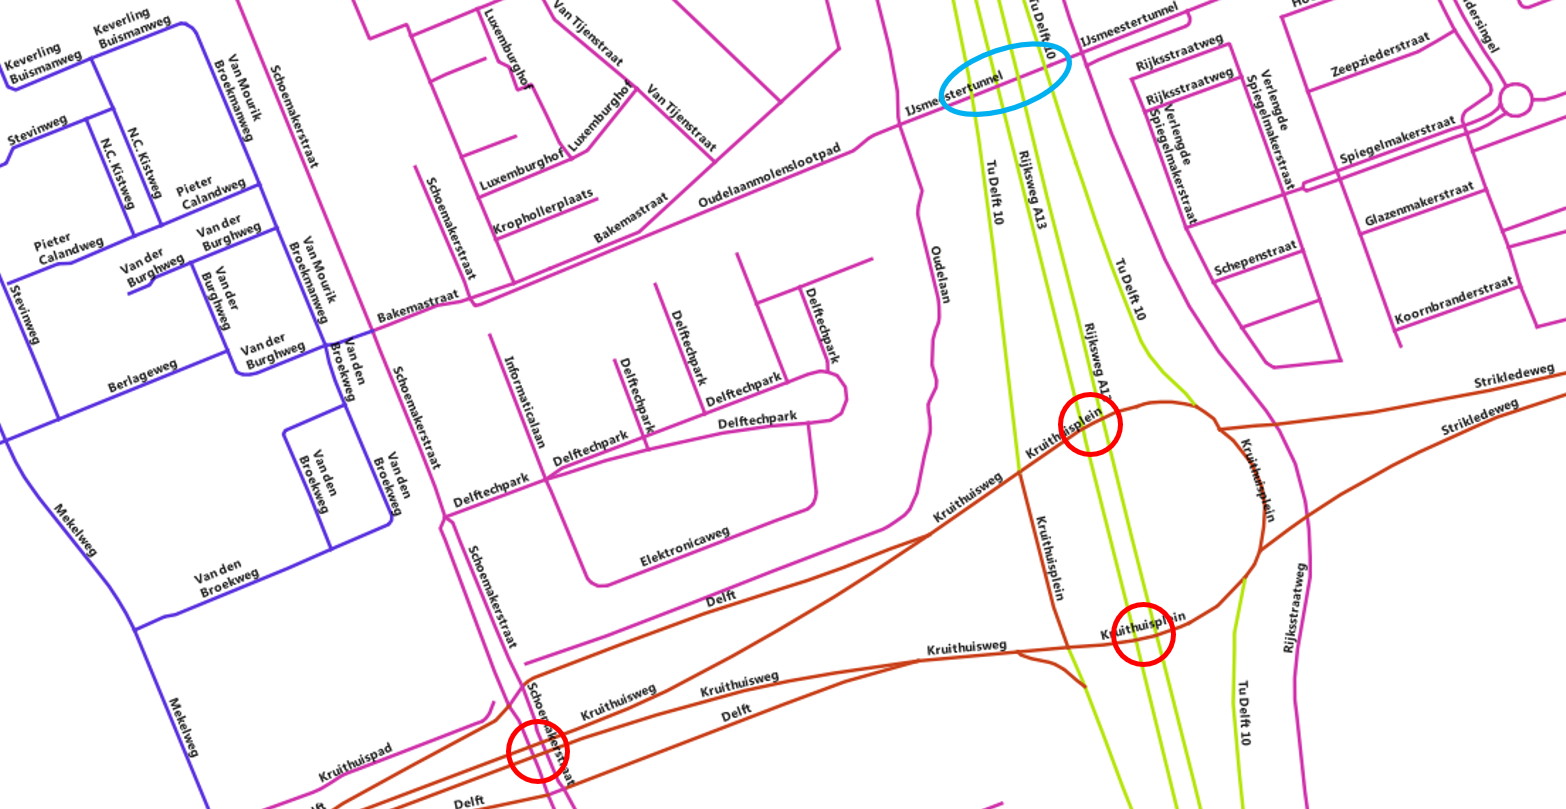
\includegraphics[width=\linewidth]{final_report/figs/nwb_sample_02.png} 
    \caption{An example render of \ac{nwb}, colour-coded to indicate the owner.}
    \label{fig:nwb}
\end{figure}

\ac{nwb} (or more specifically, NWB-Wegen, the \ac{nwb} roads product) is a vector dataset comprised of a semantically enriched set of 2D LineString objects released in the \textit{ESRI Shapefile} format. The LineStrings - dubbed \textit{wegvakken} in the documentation - are interconnected in such a way that \ac{nwb} can be regarded topologically as a graph representation of the Dutch road network. Although \ac{nwb} contains all named and numbered roads in The Netherlands, we are only interested in roads that are semantically marked as state-owned or province-owned (\ac{r_roads} and \ac{p_roads} respectively), because the new noise regulation only concerns these types. The \ac{nwb} product is managed by \ac{ndw}, but it is owned by \ac{rws} (\ac{ndw} being a division of \ac{rws}).

\ac{nwb} and the road types it contains are illustrated in Figure \ref{fig:nwb}. Yellow is used for \ac{r_roads}, red denotes \ac{p_roads} and magenta means \ac{g_roads}. \ac{w_roads} are not shown in this figure. Blue roads are roads which do not fall into the above 4 categories, in this case they are managed by the TU Delft. This render also contains examples of challenging 3D relationships. Where the provincial road Kruithuisweg crosses the municipal road Schoemakerstraat and the motorway A13, no intersection occurs in 2D because the roads cross over one another in 3D. These locations are indicated in the figure by red circles. Furthermore, where the bike path IJsmeestertunnel (a municipal road in \ac{nwb}) crosses the A13, a series of 3 short tunnels are located in reality. This is indicated in the figure by a blue oval. Although not all these road types are relevant to this project, the 3D relationships represented by these examples still are.

In addition to representing the topology of the road network, the \ac{nwb} lines are georeferenced with mediocre accuracy to also represent its approximate spatial layout. The quality description includes only a single figure, which is 5 m accuracy at 95\% confidence, i.e. two standard deviations from the mean. It is not described in any detail, how the accuracy is evaluated for each road, for instance whether it is based on the accuracy of the vertex locations of the road, an arbitrary sampling along their length, and how exactly these are aggregated into the error figure. Furthermore, we do not know whether the reference for the accuracy assessment was empirical (surveyed control points) or whether it is purely theoretical and is based on the sources and the methods involved in creating and updating the dataset.

Adding to the uncertainty is the fact that both the topological and the geographical information content of \ac{nwb} is assembled from a wide range of providers ranging from large national providers such as \ac{rws} and Kadaster, to local providers such as specific road authorities and civil engineering agencies. No clear indication is given in the documentation about the sources used for the compilation of specific \ac{nwb} road types or the estimation of their accuracies, but it is mentioned that they are not the same (\cite{nwb_docs}).

In interpreting the 5 m accuracy, it is important to note that the \ac{nwb} lines represent road centrelines, but not of the whole paved surface. The centrelines in \ac{nwb} approximate the centre of the traffic-occupied parts the roads, excluding hard shoulders and other paved surfaces connected to the road. It is also important, that \ac{nwb} often does not contain vertices for more than 200 m based on my inspection (where roads are relatively straight), and even in sharp bends for up to 20-30 m at a time. Especially in bends, this circumstance, combined with the official error figure, means that \ac{nwb} often leaves the traffic occupied road surfaces, and sometimes even the paved areas. I confirmed this problem by comparing \ac{nwb} with \ac{dtb}, \ac{ahn3}.

One such comparison is shown in Figure \ref{fig:ahnnwb}. \ac{ahn3}'s ground points are coloured blue in this figure, and \ac{nwb} centrelines are shown in white. As they have no elevation, they appear below \ac{ahn3} points and are consequently masked out partially by them. I shifted them to match \ac{ahn3}'s mean elevation locally, to make them better comparable. Comparisons such as these reveal that \ac{nwb} gets close to the edges of the paved surfaces quite often, and sometimes even leaves their surface. In sharp bends, this is made worse by the angularity introduced by the coarse lengthwise discretisation of \ac{nwb}, for instance in the location pointed out by the green arrow. In later stages of the project, I made further comparisons with \ac{bgt} and with orthoimagery (Luchtfoto 2020 from Kadaster), discussed in Section \ref{sub:completeness} and with an example shown in \ref{fig:bgtcomparison}. These comparisons further confirmed the issues.

Although the above nominal accuracy and its description are certainly not good enough for compliance with the new noise regulations, the 3D conversion of \ac{nwb} is not concerned with improving it – in fact, it is a requirement of the project not to displace \ac{nwb} horizontally. Hence, we may say that the intended outcome of the 3D conversion is to devise a method that can produce accurate elevations for \ac{nwb} \textit{assuming} that its accuracy complies with the requirements set by the new noise regulations - 20 centimetres at 95\% confidence. To achieve this compliance in practice, lateral refinement is being carried out in a separate project by matching \ac{nwb} roads with their counterparts in other, more accurate datasets. Specifically, \ac{dtb} is being used for this purpose, as well as another open data dataset called \ac{bgt}. As these datasets are already theoretically compliant with the accuracy requirements, correcting \ac{nwb} geometries based on them will foreseeably solve the lateral accuracy problems of \ac{nwb}. However, at the time of writing of this report, the \ac{bgt}-based correction has only been released for municipality-owned roads (category G for Gemeente - not relevant to us), while the \ac{dtb}-based corrections for motorways are still being finalised. Consequently both the commercial and the scientific 3D-NWB project still rely on \ac{nwb} data that lacks this correction (\cite{nwb_gecorrigeerd}).

Regardless of improving \ac{nwb}’s lateral accuracy not being within the scope of this project, it is important to be aware of it, because of its implications when overlaying \ac{nwb} with \ac{ahn3} and \ac{dtb} in the processing part of this research. The problems caused by it and the necessary workarounds are discussed in-depth in the relevant sections of the next chapters.

The \ac{nwb} product is updated every month with particular attention to always including new roads, removing outdated (demolished or permanently closed) roads and updating refurbished roads as necessary. This frequency means that \ac{nwb} is always up-to-date with changes to the road network, at least to the extent where navigation (in e.g. Google Maps, which uses \ac{nwb}) can take place without any disruptions. However, this does not mean that \ac{nwb} has a temporal resolution of one month; for that to be true, all roads would need to be re-measured every month. The monthly releases merely mean that effort is concentrated into releasing known changes to the road network frequently. Since no physical phenomena exists that would move the roads laterally (without human intervention) by a significant distance, this does not cause issues in practice.

\begin{figure}
    \centering
    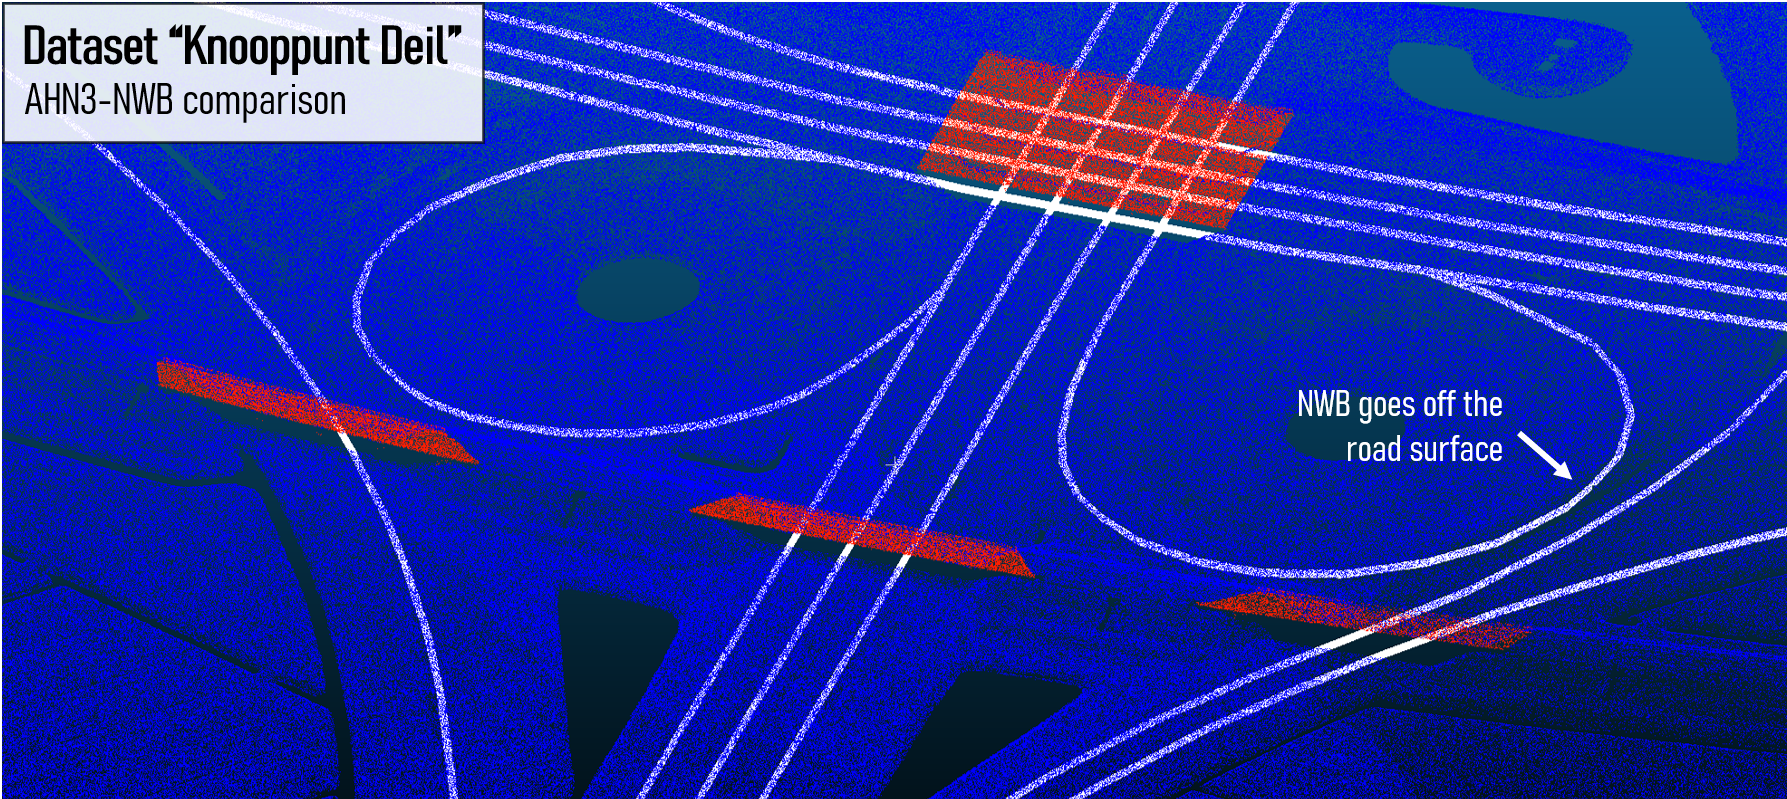
\includegraphics[width=\linewidth]{final_report/figs/ahn_sample_04_a.png} 
    \caption{Render comparing \ac{ahn3} with the relevant 2D \ac{nwb} centrelines.}
    \label{fig:ahnnwb}
\end{figure}

\subsection{Actueel Hoogtebestand Nederland – AHN}
\label{sub:ahn}

\ac{ahn} are \ac{als} datasets available as open geospatial data in The Netherlands. The surveys are commissioned every few years with \ac{ahn} (the first version) to \ac{ahn3} already complete (1996 to 2019), and the first AHN4 tiles nearing release. At this stage of the project, we are interested only in \ac{ahn3}, as it is te most recent iteration of this product. The \ac{ahn} product is owned and managed by \ac{rws}.

The dataset has a combined systematic and stochastic elevation error of 15 centimetres at two standard deviations (i.e. 95 \% confidence), and 6 to 10 points per square metre point density on average, corresponding to a 0.32 to 0.41 metre posting distance. The lateral error is 18 centimetres at two standard deviations (\cite{ahn_kwaliteit}). Comparing these to the descriptors of Lidar datasets used in the research examined as part of our literature review (see the Relevant work section), we may assert that \ac{ahn3} can be considered accurate, and to have excellent point density. It is especially accurate and dense relative to the older Lidar datasets that are mentioned in these papers, including the first iteration of \ac{ahn}.

The \ac{ahn3} point cloud has been classified semi-automatically with similarly excellent accuracy and is released with the classification included. This means that for most purposes, the point cloud needs not be ground filtered by users, and that extracting certain features is made far easier. Of the various classes available, we are interested in class 2 the most, which corresponds to ground points, and class 26 which contains, among other things, bridge structures and the roads that are found on them.

Ground points are primarily interesting to us because they contain the points reflected from land-based roads. This includes roads that were constructed directly on the terrain, as well as roads constructed on altered terrain, such as elevated ground or open trenches. It also contains the points that represent the terrain in the vicinity of the roads. Elevated roads and bridges are not considered ground points and are generally represented by gaps in class 2, which can, in most cases, be filled by using data from class 26, as shown in Figure \ref{fig:ahnbridges}. The white colour corresponds to ground points (class 2), red corresponds to bridges (class 26). All other classes were removed. The shapes of motorway lanes and ramps, as well as bridges are clearly defined. Road constructed on elevated ground is reliably classified as ground, bridges are cleanly split off by the classification. Even under thin bridges, data becomes gradually sparser at the border and becomes extinct directly below the bridge. This render also makes it clear that wherever vehicles were encountered on ground-based roads, the sampling is worse locally. It does not \textit{generally} go entirely extinct however, as most locations have been scanned multiple times. Data gaps are only observed where slow or stationary vehicles wer encountered.

Class 26 also contains other types of objects, for instance large motorway signs arching over road surfaces, as well as the civil engineering structures of elevated roads and bridges (in addition to the road surfaces on them). Reflections from vehicles transgressing bridges are also present in this class. Figure \ref{fig:ahnsigns} shows a render from the same location as \ref{fig:ahnnwb} and \ref{fig:ahnbridges}. The full-width motorway signs are clearly visible above the motorway lanes, coloured red because they originate from class 26. It also shows that the presence of water results in holes (the dark, linear features running parallel with the motorway in this render) in the ground-only point cloud. In this render, it is also visible that in my testing datasets, all points falling outside a 150-metre buffer zone around the \ac{nwb} centrelines were removed (see more information on this in Section \ref{sub:testingdata})

\begin{figure}
    \centering
    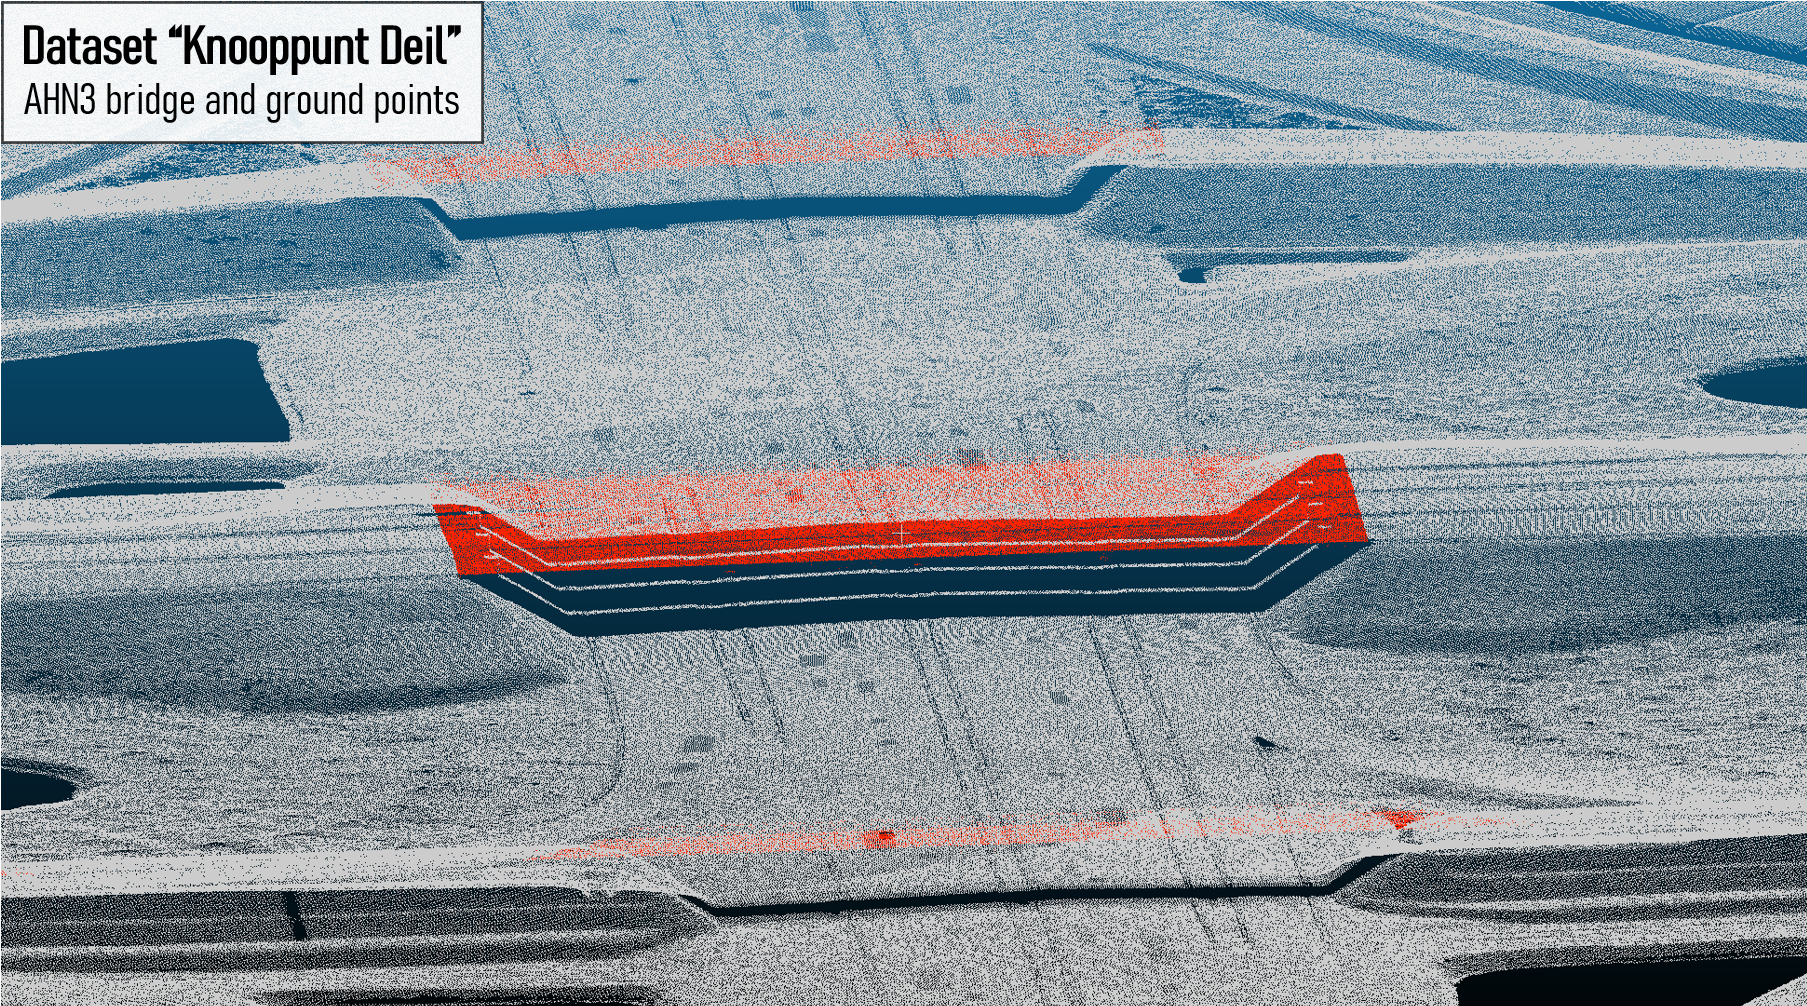
\includegraphics[width=\linewidth]{final_report/figs/ahn_sample_01.png} 
    \caption{Example render of \ac{ahn3} at Knooppunt Deil, SW of Geldermalsen, showing ground points and bridges.}
    \label{fig:ahnbridges}
\end{figure}

\begin{figure}
    \centering
    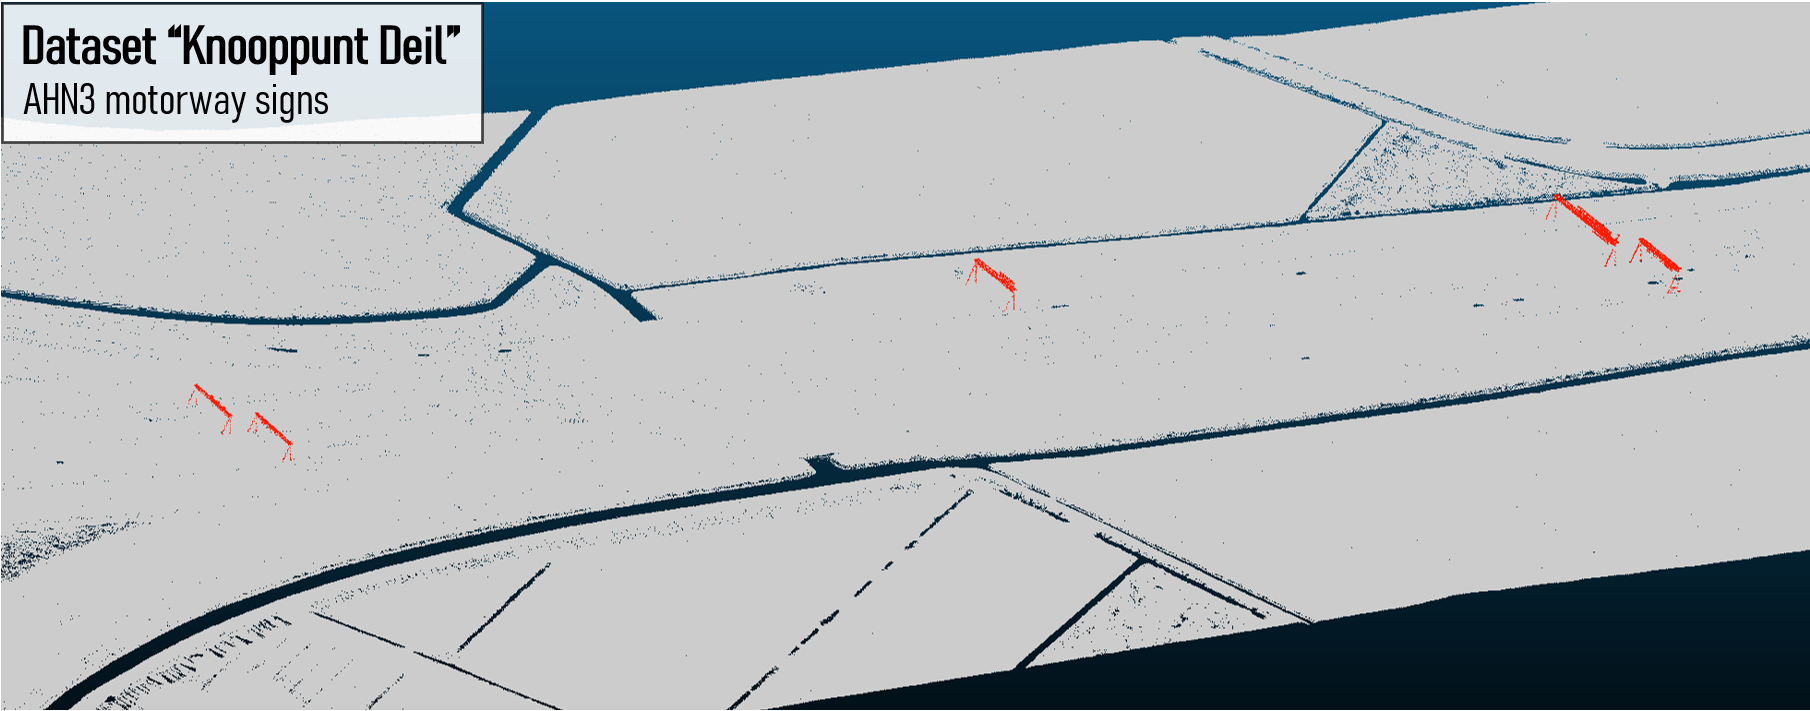
\includegraphics[width=\linewidth]{final_report/figs/ahn_sample_02.png} 
    \caption{Example render of \ac{ahn3} at Knooppunt Deil, SW of Geldermalsen, showing ground points and motorway signs.}
    \label{fig:ahnsigns}
\end{figure}

\ac{ahn3} is released in the form of a point cloud, as well as DSM and \ac{dtm} rasters. Both were produced using basic radial \ac{idw} interpolation with a fixed parametrisation. The \ac{dtm} was generated by including only points from class 2 in the interpolation step. They are available at 0.5-metre and 5-metre resolutions, with the 0.5-metre resolution being relevant to this project in terms of the target accuracy. For context, this raster converts (on average) 1.5 to 2.5 points into a single raster cell based on \ac{ahn3}'s nominal sampling density. The commercial implementation uses these rasters, as explained in Section \ref{sub:commercialproduct}.

The Lidar tiles are released in the binary LAZ format (compressed LAS, or LASzip), and are generally several gigabytes in size. As each tile only covers an approximate area of 32 square kilometres and the LAZ compression ratio for this dataset is 0.1 on average, scaling considerations are relevant to this project if the implementation is to be capable of fully converting \ac{nwb} to 3D using the raw point clouds rather than the rasters.

\subsection{Digitaal Topografisch Bestand – DTB}
\label{sub:dtb}

Like \ac{nwb}, \ac{dtb} (or more specifically, DTB-Droog, the \ac{dtb} product relevant to roads) is a Dutch open data geospatial dataset in the \textit{ESRI Shapefile} format. For the purposes of this project, we only need only those \ac{dtb} line features, which correspond to street surface markings, hence we can also regard this as a dataset comprised exclusively of LineString objects, making it identical to \ac{nwb} in its data structure apart from being a 3D dataset. \ac{dtb} is also managed by \ac{rws} and it is concerned only with state-owned roads and roads on state-leased land, which translate almost exclusively to \ac{nwb} \ac{r_roads}, that is, motorways. \ac{dtb} is, hence, not a reliable source of information about provincial roads elevations (\ac{nwb} \ac{p_roads}), our other road type of interest.

There are various types of \ac{dtb} road markings that are of interest to us, the main one being a category called \textit{verflijnen}. These \ac{dtb} lines represent the painted lines marking the outermost edges of the area open to traffic. This is a lucky correspondence with \ac{nwb}, as it too, contains the centrelines of the areas of roads that are open to traffic. The other two types I found to be reliably represent road surface elevations are the categories \textit{verfstippellijn} and \textit{blokmarkering}, which are lane separation lines and block marks respectively. The category \textit{lijnverlichting} also appeared to be interesting at first, as it corresponds to road surface lighting features (not street lighting). However, I found it to not be reliably located on road surfaces in practice, hence I excluded it from further consideration.

\begin{figure}
    \centering
    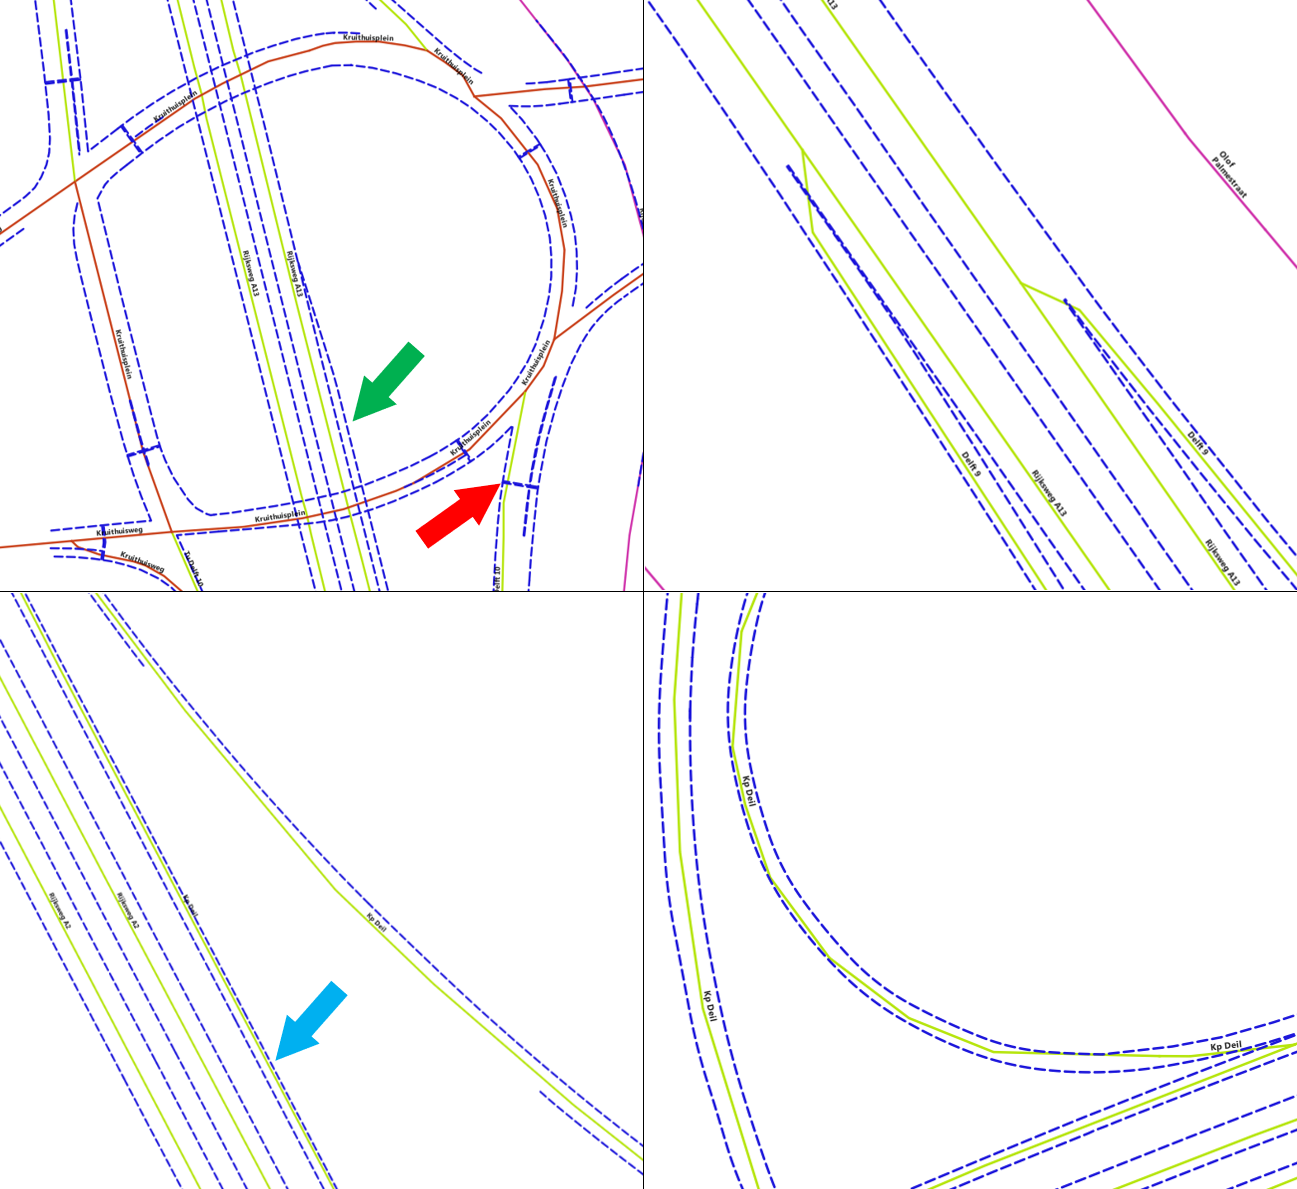
\includegraphics[width=0.95\linewidth]{final_report/figs/dtb_sample_07.png} 
    \caption{Renders of \ac{dtb} \textit{verflijnen} overlain with \ac{nwb} centrelines, illustrating "compatibility issues" and individual \ac{dtb} issues.}
    \label{fig:dtbnwb}
\end{figure}

Figure \ref{fig:dtbnwb} shows a visual comparison with \ac{nwb}, illustrating various types of significant issues that primarily stem from \ac{nwb}'s crude georeferencing. \ac{nwb} symbology is identical to that which I used in \ref{fig:nwb}, and blue dashed lines are the \ac{dtb} lines. Only \textit{verflijnen} are present in \ac{dtb} in these locations. The image in the top left shows that in practice \ac{dtb} contains many road markings, rather than just one on either side of \ac{nwb}. The illustration in the top right shows that \ac{nwb} motorway ramps often merge with the motorway lanes at unrealistic angles, causing \ac{nwb} to intersect the \ac{dtb} edge markings at these locations. The image in the bottom left illustrates that while in some places there are many \ac{dtb} road edges, in other places they are incomplete or missing entirely. Furthermore, \ac{nwb} centrelines may also get very close to \ac{dtb} edges outside of sharp bends and motorway ramps, as indicated by the blue arrow. In the bottom right, the figure shows that \ac{nwb} discretisation and inaccuracy leads to angular angular lines in sharp bends. \ac{nwb} often gets close to, or even intersects \ac{dtb} in such places.

Like \ac{nwb} (but unlike \ac{ahn3}), \ac{dtb}’s production pipeline also concerns several organisations performing various types of sensing, which are then semi-automatically assembled into the complete \ac{dtb} product. While many \ac{dtb} features are photogrammetry-derived, road surface markings are mainly from accurate land-based manual surveys or extracted from car-mounted \ac{mls} data (\cite{oudeElberink_vosselman_2012}). The documentation of \ac{dtb} consists of its formal specifications (\cite{dtb_docs}) and a handbook (\cite{dtb_handbook}). The former contains the accuracy-related details, reporting 10 cm vertical and 5 cm horizontal standard deviations, or 20 cm and 10 cm at 95\% confidence to make it comparable with the reported accuracy of \ac{nwb} and \ac{ahn3}.

Theoretically, \ac{dtb} is not only accurate, it also has a good temporal resolution. It is updated multiple times a year, specifically to always be up-to-date in terms of newly constructed roads and refurbished roads - just like \ac{nwb}. This update frequency is comparable to that of \ac{nwb}, which is part of the reason why it forms part of the commercial solution. The other part of the reason is, that it theoretically always contains data for occluded roads, even in tunnels. This means that the combined information content of \ac{dtb} and \ac{ahn3} theoretically amount to having complete coverage of the Dutch road network. Because of the ease with which elevations can be extracted from \ac{dtb} to be used in the 3D conversion of \ac{nwb} (especially considering the crudeness of \ac{nwb}'s georeferencing) prompted \ac{ndw} to consider \ac{dtb} as its \textit{primary} dataset, wherever it is available.

In practice, I found evidence to support that the above decision is fundamentally flawed, already during the input assessment stage of my project. There are places where \ac{dtb} lives up to the above \textit{theoretical} standards, but this is not the case in most of the areas I examined. Even in terms of motorways, \ac{dtb} is often incomplete to the extent that it lacks coverage over tens of kilometers. Even where it exists, its coverage may be patchy, especially in sharp bends. An example is shown in Figure \ref{fig:dtbnwb}. Commonly it only contains a single line rather than the theoretical minimum of three (two edge markings and one separation line). The separation line is the one I observed to be missing the most frequently.

Furthermore, already by considering the update methodology of the dataset, one may remark that some of the elevation measurements in it must be very outdated. Indeed, most of them are almost as old as the roads themselves, meaning that they were taken more than 20 years ago. This is where it comes into play that the update methodology of \ac{nwb} and \ac{dtb} does not really represent a high temporal resolution. In the absence of a physical phenomenon causing significant lateral ground motion, this does not cause problems with \ac{nwb}, but there \textit{is} one that may move roads up or down: subsidence. Although the surface load due the weight of the road and passing vehicles may play a role, subsidence is primarily caused by natural, geological processes. In some parts of The Netherlands, groundwater and natural gas extraction may also play a role. Although this work does not specifically study the correlation between subsidence and problems with \ac{dtb}, there is little else with which the 0.5 to 1 m differences between \ac{ahn3} and \ac{dtb} could be explained. The \ac{ahn3} measurements are at least 15 years more recent than the oldest ones in \ac{dtb}, which is where the biggest differences can be observed in elevation, as one would expect from subsidence.

Interestingly, the opposite can also be observed, although less commonly, and in a highly localised manner. In some places, \ac{dtb} is above the road surface measurements of \ac{ahn3} by a significant margin, often by more than 0.5 m. While subsidence cannot be used to explain these disagreements, there is evidence to support that the elevations in \ac{ahn3} are indeed correct and the ground has shifted upwards noticeably. The latest subsidence survey of The Netherlands reported positive changes in addition to the decreasing elevations that are associated with subsidence. I primarily observed \ac{dtb} to be below \ac{ahn3} where this map indicates negative elevation changes, and above in regions where no changes or slightly positive changes were observed in the subsidence study, verifying my hypothesis.

Figure \ref{fig:dtbahn} shows renders of \ac{dtb} overlain on \ac{ahn3} with all \ac{dtb} features shown (above), and with only \textit{verflijnen} shown (below). Ground points are shown in green. The top render illustrates that other features, such as roadside slopes, canals, ditches, safety rails are represented in \ac{dtb}. Full-width motorway signs are also occasionally represented (either by lines on the road, or on the structure itself). The bottom render shows that locally, the edge markings are in good agreement with \ac{ahn3} visually, and are only occasionally incomplete. This location has the best vertical correspondence with \ac{ahn3}, and also the best completeness, of all the areas I examined. For illustrations of the \textit{disagreements} between \ac{dtb} and \ac{ahn3}, please refer to Figure \ref{fig:lidarsegmentation1} and the associated discussion in Chapter \ref{chap:r}.

\begin{figure}
    \centering
    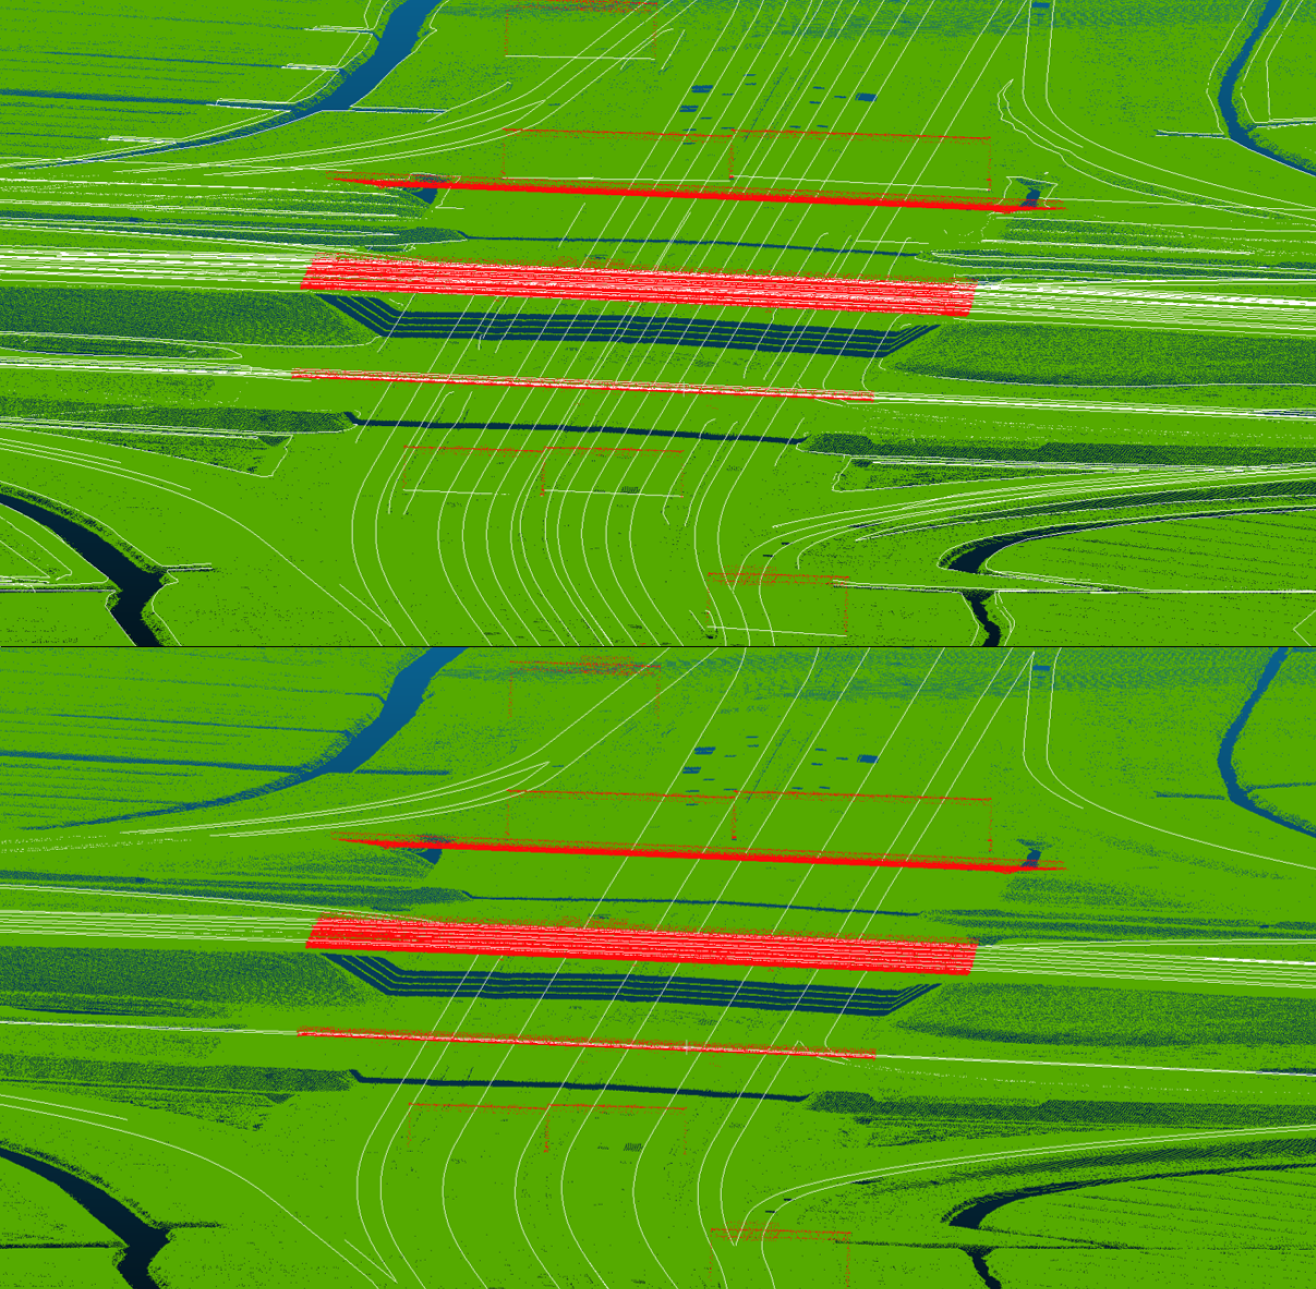
\includegraphics[width=\linewidth]{final_report/figs/ahn_sample_10.png} 
    \caption{Renders of \ac{dtb} all line features (above) and \textit{verflijnen} only (below) overlain with \ac{ahn3} in 3D.}
    \label{fig:dtbahn}
\end{figure}

\section{Methods of existing implementations}
\label{sec:methodsexisting}

\subsection{NDW prototype}
\label{sub:ndwprototype}

\ac{ndw} themselves produced a prototype implementation, which can achieve a 3D enrichment of \ac{nwb} with only a few gaps in the produced elevation profiles. Although their workflow does not have a formal documentation, I have been given a verbal description of it, as well as the output. Based on my understanding of these, their primary technique involved snapping close-by \ac{ahn3} Lidar points to the line geometries of \ac{nwb}. Notable problems with the implementation included non-road points being snapped to centrelines, causing road centrelines to be given overestimated elevations, in turn resulting in abrupt spikes in the elevation profiles.

Furthermore, no close-by points could be found for underground roads (i.e. tunnels), and strongly occluded parts of roads. For small gaps, this was resolved partially by writing an algorithm to interpolate linearly inside \ac{nwb}, using the closest vertices where snapping was successful. For larger gaps, an attempt was made to resolve issues by including information from external sources semi-automatically. Neither issue could be fully resolved via these approaches, hence the results of this project were only used by \ac{ndw} to gain a better understanding of the problem and the expected challanges. For the development of a reliable digital toolbox they subsequently commissioned a commercial implementation from \ac{rhdhv}.

\subsection{RHDHV's commercial implementation}
\label{sub:commercialproduct}

\ac{rhdhv} developed their implementation in parallel with the planning of the present scientific research. During this time, I attended \ac{ndw}-\ac{rhdhv} meetings, discussed the commercial system design and implementation details directly with \ac{rhdhv} personnel, and was granted access to the codebase of the project. Understanding their implementation was crucial for the planning and realisation of my research, as it was among my goals to estimate the effectiveness of the commercial implementation's methods, as well as assess the quality estimate the accuracy of the their final results. In addition, creating my system design while learning about the known and suspected shortcomings of their methods allowed me specifically focus on areas where a different, less pragmatic approach could yield better results.

\subsubsection{Overview of system design}

First, where \ac{nwb} vertices are too sparse, vertex densification takes place; i.e. additional vertices are created inside \ac{nwb} line segments until all vertices are found less then a certain threshold distance from their neighbours. From then onwards, \textit{different} workflows are initiated for \ac{r_roads} and \ac{p_roads}.

For \ac{p_roads} (where \ac{dtb} data does not generally exist), the workflow is conceptually similar to the one in the prototype, with the notable difference of using \ac{ahn3} \ac{dtm} rasters rather than the point cloud. Because \ac{ahn3} \ac{dtm} rasters are badly affected by both large holes and small groups of missing pixels (due to the fixed-parameter \ac{idw} interpolation that was used to generate them), \ac{rhdhv} could only make use of them by filling in the gaps of the raster using linear interpolation in a 3D \ac{tin} created from extruded raster pixel centres. They then simply interpolated elevations for \ac{nwb} from the raster using bilinear interpolation. Intermediate results of this procedure are shown on the right in \ref{fig:rhdhv}. It shows a raster being overlain with \ac{nwb} to yield elevation values. The raster still contains the holes that \ac{ahn3} rasters contain by default; these are filled in before interpolating elevations for \ac{nwb} but are shown here for demonstration purposes. Two types of holes generally occur: small-scale ones due to objects such as street furniture, vehicles and vegetation, and large ones that are typically due to large-scale occlusion due to buildings or bridges (as in this case). The test build shown here used \ac{ahn2} rasters, but their production implementation uses \ac{ahn3}.

\begin{figure}
    \centering
    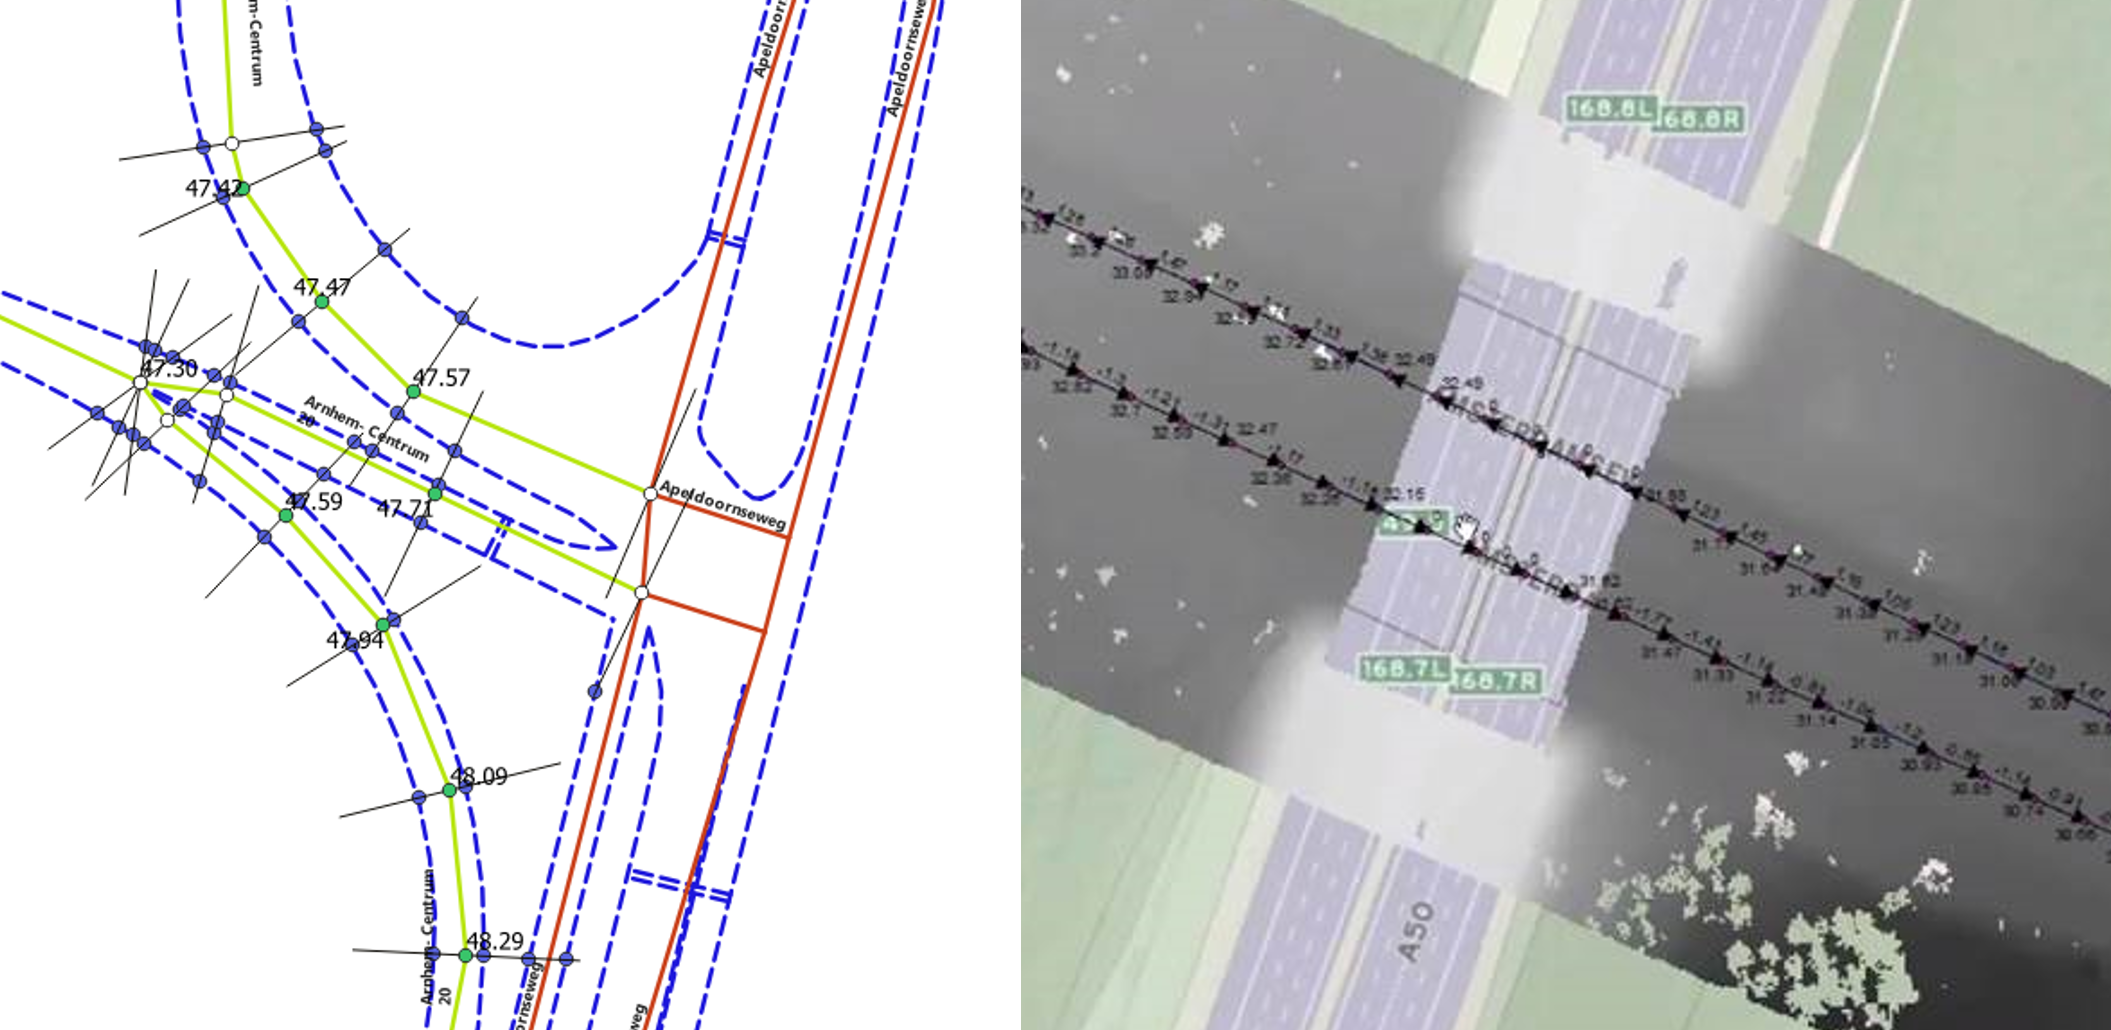
\includegraphics[width=\linewidth]{final_report/figs/rhdhv_combined.png}
    \caption{Illustrations of \ac{rhdhv}'s procedures to convert \ac{nwb} to a 3D dataset.}
    \label{fig:rhdhv}
\end{figure}

For \ac{r_roads}, \ac{dtb} is available, and the assumption is made that it is more accurate than \ac{ahn3} (or at least the stock \ac{dtm} tiles generated from \ac{ahn3}), to the extent where it should be the primary source of elevation data. Priority is thus always given to it in the procedure, with \ac{ahn}-based interpolation used only as a fallback mechanism in case \ac{dtb}-based height estimation fails for any reason (anomalous elevations computed, or missing \ac{dtb} geometry).

The goal of the underlying algorithm is to find the closest, roughly parallel \ac{dtb} line segments at any \ac{nwb} vertex, and to deduce elevations from them. First, 2D cross-sections are constructed on \ac{nwb} vertices, with each given the mean azimuth of the two \ac{nwb} line segments that they are part of, and then rotated 90 degrees. For vertices created during densification, this simply means the rotated azimuth of their parent line segment. \ac{dtb} lines are then intersected with the cross-sections and for each cross-section, the closest \ac{dtb} line that satisfies a relative angle condition is picked on both sides of \ac{nwb}. Elevation is then first linearly interpolated inside the two chosen \ac{dtb} segments to yield values exactly at their intersections with the cross-section. Lastly, elevation is interpolated linearly along the cross-section itself to yield the final elevation at the location of the \ac{nwb} vertex.

The angle condition I mentioned above is a threshold-based evaluation concerning the angle between intersected \ac{dtb} line segments and the cross-sections, and is used to ensure that the chosen \ac{dtb} segment is indeed roughly parallel to \ac{nwb} locally. This helps ensure that the algorithm does not accidentally choose a \ac{dtb} line segment that belongs to a different (underlying or overlying) road surface. The assumption is thus made that the \ac{dtb} line segments representing surface features of a given road are roughly parallel with the relevant \ac{nwb} centreline, and lie close to them. Implicitly, this also assumes that even if no other \ac{dtb} road markings are present, \ac{nwb} centrelines will still lie between two \ac{dtb} road \textit{edge} markings, i.e. \textit{verflijnen}.

In practice, backup mechanisms needed to be implemented because these assumptions do not always hold. Primarily, this is because in sharp bends \ac{nwb} may not be parallel with the relevant \ac{dtb} lines locally, and because it is frequently not complete enough to be used for the above operations. To bridge these issues, wherever the algorithm only finds a suitable \ac{dtb} intersection on \textit{one} side of \ac{nwb}, it is only that side from which the elevation value is deduced. If no suitable intersection can be found whatsoever, the \ac{ahn3} raster-based interpolation is used instead (the same workflow that is always used for \ac{p_roads}).

This procedure is illustrated on the left in \ref{fig:rhdhv}. The cross-sections that are constructed on \ac{nwb} vertices are shown as black lines. Green circles denote those vertices where the cross section could be properly intersected with \ac{dtb} lines (blue circles) and thus be given an elevation value. White circles denote where the procedure failed, and \ac{ahn} raster-based interpolation was necessary. This render illustrates that in sharp bends the assumption that \ac{nwb} and corresponding \ac{dtb} lines are parallel does not necessarily hold, because of how coarse and inaccurate \ac{nwb}'s georeferencing is, especially relative to \ac{dtb} which is very accurate horizontally. The render also illustrates that \ac{p_roads} are not processed in this way, not even if they have \ac{dtb} lines next to them (which frequently occurs in the vicinity of motorways).

\subsubsection{Potential limitations}

At the time of finalising this report, the preliminary results of the commercial implementation have already been made public, as described in \cite{nwb_hoogte}. In this section I discuss the \textit{suspected} limitations of their methods, not yet the properties of their results. These will only be discussed in the context of the comparison of the two sets of results. During the project planning, system design and implementation stages, the commercial results were not yet available and as a result, the bulk of my work - almost everything apart from Section \ref{sec:r_comparison} - is based on verbal descriptions of their methods and the commercial source code.

First and foremost, I suspected that using \ac{ahn3} rasters in place of the point cloud would affect the quality of their conversion. Point cloud to raster conversion is, by definition, associated with inherent information loss (less raster cells than point cloud points), and further reduction in accuracy is introduced by the interpolation mechanism itself, that created the rasters. Radial \ac{idw} was used to generate \ac{ahn3} \ac{dtm} tiles, which several of the reviewed papers found to be specifically unsuitable for interpolating large-scale areas in which zones of decreased point density or gaps exist – both of which characterise ground-filtered \ac{ahn} data (e.g. \cite{guo_etal_2010}). In addition, the procedure performs another layer of interpolation to infill gaps, which may further deteriorate accuracy. Furthermore, \ac{rhdhv} uses bilinear interpolation inside the raster to produce \ac{nwb} elevations, which is suggested by \cite{shi_etal_2005}, to be less accurate than other common methods such as bicubic.

Furthermore, there is no mechanism built into the software to deal with occlusion in the case of \ac{p_roads}, and also \ac{r_roads} where \ac{dtb} is unavailable. This means that wherever \ac{nwb} elevations are interpolated in occluded road segments from \ac{ahn3} rasters, they will be incorrect. Just like in the \ac{ndw} prototype, these values will show up as spikes in the elevation profiles, as well as longer bumps where wide features (e.g. bridges) are encountered. Since there is no outlier filtering or smoothing algorithm built into the software either, the severity of this issue is not mitigated in any way.

Based on the input assessment, it is also evident that prioritising \ac{dtb} wherever it is available may itself be a questionable decision, in view of the fact that the output's accuracy needs to measure up to the noise regulation's expectations, at least theoretically. \ac{dtb} is accurate horizontally, in fact it is theoretically more accurate than \ac{ahn3}. However, even if its vertical accuracy was also satisfactory at the time of its acquisition, it no longer is, due to various degrees of vertical ground motion taking place in the country. As elevations in \ac{dtb} are not updated where no civil engineering changes have taken place in the road network, its road surface markings are often far too outdated to be used with any certainty, especially considering that there is no reason to do so given that \ac{ahn3} contains equally accurate, but significantly more recent data.

Lastly, the commercial implementation lacks a formal accuracy assessment. Although this is common with comparable commercial products, in this case the output dataset needs to comply with formal accuracy \textit{requirements}. Without a quantitative or at least qualitative accuracy assessment of some form, there is not enough evidence to support the applicability of the commercial results to the noise modelling applications they are intended for.

Since the accuracy of \ac{ahn3} rasters is known and simple bilinear interpolation is used to obtain elevations from them, deriving output accuracy would not be difficult wherever their solution uses \ac{ahn3}. This excludes interpolating in gap-filled pixels, which would need further considerations. In the case of \ac{dtb}, the evaluation of accuracy may be equally simple, as the underlying computations all boil down to linear interpolation. However, wherever \ac{dtb} data is old, any accuracy quantification would be meaningless because \ac{dtb} itself does not comply with its own formal accuracy, due to vertical land motion.